% arara: pdflatex
% arara: pdflatex
% --------------------------------------------------------------------------
% the CNLTX bundle
%
%   LaTeX source code and output
%
% --------------------------------------------------------------------------
% Clemens Niederberger
% Web:    https://github.com/cgnieder/cnltx/
% E-Mail: contact@mychemistry.eu
% --------------------------------------------------------------------------
% Copyright 2013 Clemens Niederberger
%
% This work may be distributed and/or modified under the
% conditions of the LaTeX Project Public License, either version 1.3
% of this license or (at your option) any later version.
% The latest version of this license is in
%   http://www.latex-project.org/lppl.txt
% and version 1.3 or later is part of all distributions of LaTeX
% version 2005/12/01 or later.
%
% This work has the LPPL maintenance status `maintained'.
%
% The Current Maintainer of this work is Clemens Niederberger.
% --------------------------------------------------------------------------
% The cnltx bundle consists of the files
%  - cnltx-base.sty, cnltx-example.sty cnltx-doc.cls, cnltx-csnames.sty,
%    cnltx-tools.sty
%  - cnltx_en.tex, cnltx_en.pdf
%  - README
% --------------------------------------------------------------------------
% If you have any ideas, questions, suggestions or bugs to report, please
% feel free to contact me.
% --------------------------------------------------------------------------
\documentclass[load-preamble+]{cnltx-doc}
\usepackage[utf8]{inputenc}

\usepackage{varioref}

\usepackage{array,booktabs}
\usepackage{tikz}
\usetikzlibrary{chains}

\setcnltx{
  name     = cnltx ,
  title    = the cnltx bundle ,
  version  = \csname cnltx@@version\endcsname ,
  date     = \csname cnltx@@date\endcsname ,
  subtitle = Documentation for \LaTeXe\ Packages or Classes ,
  info     = \LaTeX\ examples the \texorpdfstring{\textsc{cn}}{CN} way ,
  authors  = Clemens Niederberger ,
  email    = contact@mychemistry.eu ,
  url      = https://github.com/cgnieder/cnltx ,
  abstract = {%
    A bundle of packages and classes for consistent format of control
    sequences, package options, source code with examples, writing a package
    manual (including an index containing the explained control sequences,
    options, \ldots).%
  } ,
  add-cmds = {
    % internal macros:
    cnltx@define@colorscheme,cnltx@gobble,cnltx@ifsym,
    cnltx@listings@style,cnltx@mdframed@options,cnltx@caption@font,
    cnltx@captionlabel@font,
    % official macros:
    changedversion,cls,
    cnltxat,cnltxbang,cnltxequal,
    code,codefont,command,cs,csidx,
    CTANurl,
    darg,Default,default,
    env,environment,
    inputexample,inputsidebyside,inputsourcecode,
    key,keybool,keychoice,keyval,
    marg,module,Module,
    newarg,newname,newnote,newpackagename,newinputsourcefilecmd,
    newsourcecodeenv,
    oarg,opt,option,
    pkg,
    sarg,setcnltx,sinceversion,sourceformat
  },
  add-silent-cmds = {
    at,
    carlisle,
    foothree,
    GetTranslation,
    nohyperpage
  } ,
  add-envs = {
    commands,
    environments,
    example,
    options,
    sidebyside,sourcecode
  },
  add-frame-options = {
    innerleftmargin=2em
  }
}

\newpackagename\cnltxbase{cnltx-base}
\newpackagename\cnltxexample{cnltx-example}
\newpackagename\cnltxcsnames{cnltx-csnames}
\newpackagename\cnltxtools{cnltx-tools}
\newpackagename\cnltxdoc{cnltx-doc}

\newnote*\bypackage[1]{provided by the \csname cnltx#1\endcsname\ package}
\newnote*\byclass{provided by the \cnltxdoc\ class}

\newname\oberdiek{Heiko}{Oberdiek}
\newname\egreg{Enrico}{Gregorio}
\newname\heinz{Carsten}{Heinz}
\newname\moses{Brooks}{Moses}
\newname\hoffmann{Jobst}{Hoffmann}
\newname\daniel{Marco}{Daniel}

\newcommand*\file[1]{\code{#1}}
\newcommand*\latin[1]{\textit{#1}}

\newcommand*\PDF{\cnltxacronym{PDF}{pdf}}

\newenvironment{colors}
  {%
    \def\colour##1{\item\code{\textcolor{##1}{##1}}}%
    \cnltxlist
  }
  {\endcnltxlist}

\def\at{\cnltxat}
\def\bang{\cnltxbang}
\def\equal{\cnltxequal}

\begin{document}

\part{About The Bundle}

\section{Background}

The \cnltx\ bundle contains different packages and classes.  I developed
it as a successor of my class \cls{cnpkgdoc} that I used for writing the
documentation of my packages.   The intention behind this is a cleaner
interface and less unnecessary ballast, hence the separation into packages and
classes.  The bundle provides source code environments that also print the
output and defines quite a number of macros for formatting of control sequence
names, package names, package options and so on.

Part of the motivation is also that users have asked me how I created the
manuals for my packages.  Now I can refer to this bundle.

Another reason for the splitting into separate packages is -- besides the
advantage of easier maintenance -- is that I may want to add programming tools
that I use often into \cnltxbase\ which may allow me (and others) to use them
for other packages, too, without having to define them each time.  So it is
quite possible that \cnltxbase\ will get extended in the future.

The best documentation for the bundle as always is the source code of the
\file{sty} and \file{cls} files but I'm trying to provide a documentation as
comprehensive as possible.  This is one of the reasons why this documentation
is noticeably longer than the one for \cls{cnpkgdoc}.

The bundle reflects the fact that I haven't started using literate
programming, yet.  I don't use \code{docstrip} and don't write \file{dtx}
files but always write the \file{sty} or \code{cls} files directly.  The
manual is always created parallel but separately.  While I'm entirely aware of
the advantages of literate programming I never could bring myself to start
to use it myself.  As a consequence I have no idea if this bundle can be used
for it or not.

Source code formatting is done with the help of the powerful \pkg{listings}
package by \heinz\ and later \moses, now maintained by \hoffmann.  The only
real drawback I have found with it is recognizing starred und un-starred
versions of an environment as different keywords.  This does not seem to be
possible which is why indexing of such environments will lead to wrong page
numbers.

The fancy frames of the source code examples are realized with the
\pkg{mdframed} package by \daniel, loaded with the option
\keyis*{framemethod}{tikz}.

\section{Bundled Packages and Classes}

The \cnltx\ bundle currently bundles the following packages and classes:
\begin{itemize}
  \item \cnltxbase\ -- a package that defines base macros for error-messaging,
    expansion control and tokenlist manipulation.  It also provides color
    definitions and defines a few color schemes for the \cnltxdoc\ class.  All
    other packages and classes of the \cnltx\ bundle load this package.\par
    This package can be loaded alone.
  \item \cnltxexample\ -- a package that defines macros and environments for
    describing control sequences and options and for including source code.\par
    This package can be loaded alone.
  \item \cnltxcsnames\ -- a package that defines a list of highlighted control
    sequence names, loaded by \cnltxexample.\par
    It does not make sense to load this package directly: it only defines a
    single macro containing the list of control sequence names.  The package
    only exists for maintanance reasons.\par
    The list is by no means comprehensive.  If you like to extend it feel free
    to fork the github repo (\url{\csname cnltx@package@url\endcsname}).
    That would be very much appreciated.
  \item \cnltxtools\ -- a package that defines tools used by \cnltxdoc\ that
    are unrelated to \LaTeX\ documentation \latin{per se}.
  \item \cnltxdoc\ -- a class for writing package manuals.  Loads
    \cnltxexample\ and \cnltxtools.
  \item \file{cnltx.ist} -- an index style file that is used when the option
    \option{add-index} is activated and the option \option{index-style} is not
    used.
\end{itemize}

\section{License and Requirements}\label{sec:license}
\license

The \cnltxbase\ package loads the following packages: \needpackage{pgfopts},
\needpackage{etoolbox}, \needpackage{trimspaces} and \needpackage{xcolor}.

The \cnltxcsnames\ package only loads \cnltxbase.

The \cnltxexample\ package loads the following packages:
\cnltxbase, \cnltxtools, \needpackage{translations}, \needpackage{listings},
\needpackage{mdframed} and \needpackage{idxcmds}.

The \cnltxtools\ package loads \cnltxbase\ and
\needpackage[macros/latex/contrib/oberdiek]{accsupp}.

The \cnltxdoc\ class loads the package with the same name and additionally
the following packages: \cnltxbase, \cnltxexample, \pkg{translations},
\needpackage{ulem}, \needpackage[macros/latex/required/tools]{multicol},
\needpackage[macros/latex/contrib/ms]{ragged2e}, \needpackage{marginnote} and
\needpackage{hyperref}.  It is a wrapper class for the
\KOMAScript\ class \cls{scrartcl}\footnote{\CTANurl{koma-script}}.

Like all of my packages \cnltx\ implicitly relies on an up to date \TeX\
distribution.

\part{Details of Available Commands, Environments and Options}

\section{Options and Setup}
The \cnltx\ bundle has a number of options.  The \cnltxdoc\ class only knows
a few options (described in section~\vref{sec:class:options}) as \emph{class}
options.  All other options regardless if they're defined by a package or a
class can and should be set with the setup command:
\begin{commands}
  \command{setcnltx}[\marg{options}]
    setup command for \cnltx.
\end{commands}
The source code environments defined by the \cnltxexample\ package also have
optional arguments that can be used to set the options for the environment
locally.

\section{Available Commands}
\subsection{Description of Macros, Environments and  Options}\label{sec:cmds:macros}

The commands described in this section all are provided by the \cnltx\
package\bypackage{example}.  They all are related to the typesetting of
provided macros, options and the like.

\begin{commands}
  \command{code}[\marg{arg}]
    Formatting of source code.  This is \emph{no} verbatim command.  Used
    internally in the following commands.
  \command{verbcode}[\meta{delim}\meta{code}\meta{delim}]
    \sinceversion{0.2}A verbatim command that uses the same formatting as the
    source code example environments.  This is a wrapper for \cs*{lstinline}
    which loads the corresponding style.
  \command{cs}[\sarg\marg{name}]
    Format the control sequence \meta{name}, \cs{cs}\Marg{name}:
    \cs*{name}.  Adds a corresponding index entry.  The starred form does not
    add an index entry.
  \command{csidx}[\marg{name}]
    Adds an index entry but does not typeset the control sequence
    \meta{name}.
  \command{env}[\sarg\marg{name}]
    Format the environment \meta{name}, \cs{env}\Marg{name}:
    \env*{name}.  Adds a corresponding index entry with a hint that the entry
    refers to an environment.  The starred form does not add an index entry.
  \command{envidx}[\marg{name}]
    Adds an index entry but does not typeset the environment \meta{name}.
  \command{meta}[\marg{meta}]
    Description of an argument, \cs{meta}\Marg{meta}: \meta{meta}.
  \command{marg}[\marg{arg}]
    A mandatory argument. \meta{arg} is formatted with \cs{meta} if it is not
    blank, \cs{marg}\Marg{arg}: \marg{arg}.
  \command{Marg}[\marg{arg}]
    \sinceversion{0.2}A mandatory argument. \meta{arg} is formatted with
    \cs{code} if it is not blank, \cs{Marg}\Marg{arg}: \Marg{arg}.
  \command{oarg}[\marg{arg}]
    An optional argument. \meta{arg} is formatted with \cs{meta} if it is not
    blank, \cs{oarg}\Marg{arg}: \oarg{arg}.
  \command{Oarg}[\marg{arg}]
    \sinceversion{0.2}An optional argument. \meta{arg} is formatted with
    \cs{code} if it is not blank, \cs{Oarg}\Marg{arg}: \Oarg{arg}.
  \command{darg}[\marg{arg}]
    An argument with parentheses as delimiters. \meta{arg} is formatted with
    \cs{meta} if it is not blank, \cs{darg}\Marg{arg}: \darg{arg}.
  \command{Darg}[\marg{arg}]
    \sinceversion{0.2}An argument with parentheses as delimiters. \meta{arg}
    is formatted with \cs{code} if it is not blank, \cs{Darg}\Marg{arg}:
    \Darg{arg}.
  \command{sarg}
    An optional star argument, \cs{sarg}: \sarg.
  \command{option}[\sarg\marg{name}]
    An option \meta{name}, \cs{option}\Marg{name}: \option{name}.  Adds a
    corresponding index entry.  The starred form does not add an index entry.
  \command{optionidx}[\marg{name}]
    Adds an index entry but does not typeset the option \meta{name}.
  \command{module}[\sarg\marg{name}]
    A module \meta{name}, \cs{module}\Marg{name}: \module{name}.  Adds a
    corresponding index entry.  The starred form does not add an index entry.
    In some of my package I like to organize options by grouping them in
    different classes that I call ``modules''.  This command refers to those
    modules.
  \command{moduleidx}[\sarg\marg{name}]
    Adds an index entry but does not typeset the option \meta{name}.
  \command{key}[\sarg\code{-}\marg{name}\marg{value}]
    A key \meta{name} with value \meta{value}, the optional star prevents an
    index entry, the  optional \code{-} strips the braces around \meta{value};
    \cs{key}\Marg{key}\Marg{value}: \key{key}{value};
    \cs{key}\code{-}\Marg{key}\Marg{value}: \key-{key}{value}
  \command{keyis}[\sarg\marg{name}\marg{value}]
    \sinceversion{0.2}A key \meta{name} set to value \meta{value}, the
    optional star prevents an index entry, \cs{key}\Marg{keyis}\Marg{value}:
    \keyis{key}{value}.
  \command{choices}[\marg{clist of choices}]
    A list of choices, \cs{choices}\Marg{one,two,three}:
    \choices{one,two,three}
  \command{choicekey}[\marg{name}\marg{clist of choices}]
    A key \meta{name} with a list of possible values,
    \cs{choicekey}\Marg{key}\Marg{one,two,three}:
    \choicekey{key}{one,two,three}
  \command{boolkey}[\marg{name}]
    A boolean key \meta{name} with choices \code{true} and \code{false},
    \cs{boolkey}\Marg{key}: \boolkey{key}
  \command{default}[\marg{value}]
    Markup for a default choice,
    \cs{choices}\Marg{one,\cs{default}\Marg{two},three}:
    \choices{one,\default{two},three}
\end{commands}


\subsection{Versioning Commands, Licensing and Related  Stuff}\label{sec:cmds:versioning}

The commands described in this section are provided by the \cnltx\
class\byclass\ except where indicated differently.  These commands are related
to information about the legal stuff of a package and where to find it on th
world wide web.

\begin{commands}
  \command{sinceversion}[\marg{version}]
    \sinceversion{0.0}Gives a sidenote like the one on the left.
  \command{changedversion}[\marg{version}]
    \changedversion{0.0}Gives a sidenote like the one on the left.
  \command{newnote}[\sarg\marg{cs}\oarg{num}\marg{definition}]
    Defines a note like \cs{sinceversion}.  The star makes the note macro
    short, \meta{num} defines the number of mandatory arguments.  Optional
    arguments are not possible.  \cs{sinceversion} was defined as follows:
    \verbcode+\newnote*\sinceversion[1]{Introduced in version~#1}+
  \command{newpackagename}[\marg{cs}\marg{name}]
    Define a comand \meta{cs} that prints \meta{name} formatted like \cnltx.
  \command{newname}[\marg{cs}\marg{first name}\marg{second name}]
    \bypackage{tools}Defines \meta{cs} to write out the full name and add an
    index entry sorted by the last name.  Also defines a starred variant of
    \meta{cs} that only writes the last name but still adds the full index
    entry.
  \command{lppl}
    Typesets ``\lppl'' and adds a corresponding index entry.
  \command{LPPL}
    Typesets ``\LPPL'' and adds a the same index entry as \cs{lppl}.
  \command{license}[\sarg\oarg{maintenance status}]\Default{maintained}
    \changedversion{0.2}Typesets `\license*'.  The un-starred variant adds a
    \cs*{par}.
  \command{ctan}
    Typesets ``\ctan'' and adds a corresponding index entry.
  \command{CTAN}
    Typesets ``\CTAN'' and adds the same index entry as \cs{ctan}.
  \command{cnltxacronym}[\marg{pdf and sort string}\marg{acronym}]
    \bypackage{tools}Typesets \meta{acronym} with small caps and uses
    \meta{pdf and sort string} as \PDF\ string and for sorting the index entry
    that is added.  This command was used to define \cs{lppl} and \cs{ctan}.
    \emph{This is not intended as a replacement for packages like \pkg*{acro}
      or \pkg*{glossaries}!}  In fact it is a ``poor man's'' solution that
    allows me not to require one of those packages.
  \command{pkg}[\sarg\marg{package}]
    \bypackage{example}Format the package name \meta{package} and add an
    index entry.  The starred variant adds nothing to the index.
  \command{pkgidx}[\marg{package}]
    \bypackage{example}Add an index entry for the package \meta{package}.
  \command{cls}[\sarg\marg{class}]
    \bypackage{example}Format the class name \meta{class} and add an index
    entry.  The starred variant adds nothing to the index.
  \command{clsidx}[\marg{class}]
    \bypackage{example}Add an index entry for the class \meta{class}.
  \command{CTANurl}[\oarg{directory}\marg{name}]
    Writes a \ctan\ link like the ones in section~\vref{sec:license} in the
    footnotes.  The predefined directory is \code{macros/latex/contrib}.  The
    link address will be:\par
    \code{http://mirrors.ctan.org/\meta{directory}/\meta{name}/}.
  \command{needpackage}[\oarg{directory}\marg{name}]
    \sinceversion{0.2}A wrapper for
    \verbcode+\pkg{#2}\footnote{\CTANurl[#1]{#2}}+
  \command{needclass}[\oarg{directory}\marg{name}]
    \sinceversion{0.2}A wrapper for
    \verbcode+\cls{#2}\footnote{\CTANurl[#1]{#2}}+
\end{commands}

\begin{example}
  \newpackagename{\foothree}{foo-3}%
  now \foothree\ looks like \cnltx.

  \newname\carlisle{David}{Carlisle}%
  \carlisle\ is a well-known member of the \LaTeX\ community.  \carlisle* is
  the author of many packages such as \pkg*{longtable}.
\end{example}

\subsection{Input Source Code Files}
Similar to the environments described in section~\vref{sec:envs:sourcecode}
\cnltxexample\ provides a few commands for inputting source code files,
formatting and printing the source code and inputting the file directly.
\begin{commands}
  \command{inputexample}[\oarg{options}\marg{file name}]
    The equivalent of the \env{example} environment, see
    section~\vref{sec:envs:sourcecode}.
  \command{inputsidebyside}[\oarg{options}\marg{file name}]
    The equivalent of the \env{sidebyside} environment, see
    section~\vref{sec:envs:sourcecode}.
  \command{inputsourcecode}[\oarg{options}\marg{file name}]
    The equivalent of the \env{sourcecode} environment, see
    section~\vref{sec:envs:sourcecode}.
\end{commands}

It is possible to define further commands like this:
\begin{commands}
  \command{newinputsourcefilecmd}[\oarg{option}\marg{control sequence}]
    Defines \meta{control sequence} as a new source code input command where
    \meta{options} are preset.
\end{commands}

The existing commands have been defined like this:
\begin{sourcecode}
  \newinputsourcefilecmd\inputexample
  \newinputsourcefilecmd[side-by-side]\inputsidebyside
  \newinputsourcefilecmd[code-only]\inputsourcecode
\end{sourcecode}

\section{Available Environments}\label{sec:envs}
\subsection{Description Environments}\label{sec:envs:description}
\cnltxdoc\ defines some description environments used to describe macros,
environments or options.

\begin{environments}
  \environment{commands}
    A description-like environment for describing commands.  While this
    environment is a list internally and thus recognizes \cs*{item} own
    commands are used to describe macros.  They are explained in
    section~\vref{sec:usage:commands}.
  \environment{options}
    A description-like environment for describing options.  While this
    environment is a list internally and thus recognizes \cs*{item} own
    commands are used to describe options.  They are explained in
    section~\vref{sec:usage:options}.
  \environment{environments}
    A description-like environment for describing environments.  While this
    environment is a list internally and thus recognizes \cs*{item} own
    commands are used to describe environments.  They are explained in
    section~\vref{sec:usage:environments}.
\end{environments}

These environments are lists all using the same internal \cs*{list}.  The
setup of this list can be changed via an option:

\begin{options}
  \keyval{list-setup}{definitions}{}
    \Default{\cs*{leftmargin}=0pt \cs*{labelwidth}=2em \cs*{labelsep}=0pt
      \cs*{itemindent}=-1em }
    The setup of the \cs*{list} used by the \env{commands}, \env{options} and
    \env{environments} environments.
\end{options}

\subsection{Source code Environments}\label{sec:envs:sourcecode}
\cnltxexample\ defines the following environments that are used to display
source code and possibly the output of the source code, too.

\begin{environments}
  \environment{example}[\oarg{options}]
    This environment is a formatted verbatim environment that also inputs the
    output of the inputted code.  This environment is described in
    section~\vref{sec:usage:examples}.
  \environment{sidebyside}[\oarg{options}]
    This environment is a formatted verbatim environment that also inputs the
    output of the inputted code.  Source and output are printed side-by-side.
    This environment is described in section~\vref{sec:usage:examples}.
  \environment{sourcecode}[\oarg{options}]
    This environment is a formatted verbatim environment.  This environment is
    described in section~\vref{sec:usage:examples}.
\end{environments}
  
\sinceversion{0.2}In each of these environments certain hooks are provided
that can be used to add definitions you like:
\begin{options}
  \keyval{pre-code}{definitions}
    \meta{definitions} are placed before the source code is inserted.
  \keyval{after-code}{definitions}
    \meta{definitions} are placed after the source code is inserted.
  \keyval{pre-source}{definitions}
    \meta{definitions} are placed before the output of the source code is
    inserted.
  \keyval{after-source}{definitions}
    \meta{definitions} are placed after the output of the source code is
    inserted.
\end{options}

It is possible to define further environments like this:
\begin{commands}
  \command{newsourcecodeenv}[\oarg{option}\marg{name}]
    Defines \meta{name} as a new source code environment where
    \meta{options} are preset.
\end{commands}

The existing environments have been defined like this:
\begin{sourcecode}
  \newsourcecodeenv{example}
  \newsourcecodeenv[side-by-side]{sidebyside}
  \newsourcecodeenv[code-only]{sourcecode}
\end{sourcecode}

\section{Usage}
\subsection{Command Descriptions}\label{sec:usage:commands}
Inside of the environment \env{commands} that was introduced in
section~\vref{sec:envs:description} items are input via the following command:
\begin{commands}
  \command{command}[\sarg\marg{name}\oarg{stuff after}]
    This macro formats a control sequence with \cs{cs} and puts a line break
    after it.  The optional argument allows printing things directly after the
    command name and can thus be used for adding arguments.
  \command{Default}[\sarg\code{!}\marg{code}]
    \changedversion{0.3}This command can be placed after \cs{command} or
    \cs{option}  in order to give a default definition of a macro or a default
    value of an option.  The definition will then be placed on the same line
    flush right.  The star prevents the insertion of \cs*{newline} after it.
    The optional bang adds the information that an option is mandatory,
    \latin{i.e.}, it has to be set.
\end{commands}
\begin{example}
  \begin{commands}
    \command{cs}
      This is about foo bar baz.
    \command{cs}[\marg{arg}]
      This one has an argument.
    \command{cs}[\sarg\oarg{option}]
      This has a star variant and an optional argument.
    \command{cs}\Default{foo bar}
      This one has the default replacement text \code{foo bar}
  \end{commands}
\end{example}

\subsection{Option Descriptions}\label{sec:usage:options}
The \env{options} environment knows a few more commands to meet all the
different kinds of options.
\begin{commands}
  \command{opt}[\sarg]
    An option.  The star prevents an index entry.
  \command{keyval}[\sarg\code{-}\marg{key}\marg{value}]
    A key/value option.  The optional star prevents an index entry.  The
    optional \code{-} strips the braces around \meta{value}, see the example
    below.
  \command{keychoice}[\sarg\marg{key}\marg{list of choices}]
    A key/value option where the value is one of a list of choices.  The star
    prevents an index entry.
  \command{keybool}[\sarg\marg{name}]
    A boolean key, that ist a choice key with choices \code{true} and 
    \code{false}.  The star prevents an index entry.
  \command{Default}[\sarg\code{!}\marg{code}]
    \changedversion{0.3}This command can be placed after \cs{command} or
    \cs{option}  in order to give a default definition of a macro or a default
    value of an option.  The definition will then be placed on the same line
    flush right.  The star prevents the insertion of \cs*{newline} after it.
    The optional bang adds the information that an option is mandatory,
    \latin{i.e.}, it has to be set.
  \command{Module}[\sarg\code{!}\marg{name}]
    \sinceversion{0.3}This command can be placed after \cs{option} but before
    \cs{Default} in order to determine the module the option belongs to.  It
    will be written in the left margin next to the option name.  The star
    prevents the insertion of \cs*{newline} after it.  The optional bang
    \emph{adds} an index entry for the module.  This is somehow inconsistent
    with many of the other commands where an optional star \emph{prevents} an
    index entry but it fits to the functionality of \cs{Default} which is why
    this syntax was chosen.
\end{commands}

The following demonstrates how the commands would be used to create option
descriptions:
\begin{sourcecode}
  \begin{options}
    \opt{foo}
      This makes stuff.  Let's add a few more words so that the line gets
      filled and we can see how the output actually looks.
    \opt*{foo}\Default{bar}
      This makes stuff.  Let's add a few more words so that the line gets
      filled and we can see how the output actually looks.
    \opt{foo}\Module{bar}
      This option belongs to \module*{bar}.  Let's add a few more words so
      that the line gets filled and we can see how the output actually
      looks.
    \opt{foo}\Module{bar}\Default{baz}
      This option belongs to \module*{bar}.  Let's add a few more words so
      that the line gets filled and we can see how the output actually
      looks.
    \keyval{foo}{bar}\Default
      This makes stuff.  Let's add a few more words so that the line gets
      filled and we can see how the output actually looks.
    \keyval{foo}{bar}\Default!
      This makes stuff.  Let's add a few more words so that the line gets
      filled and we can see how the output actually looks.
    \keyval*{foo}{bar}
      This makes stuff.  Let's add a few more words so that the line gets
      filled and we can see how the output actually looks.
    \keyval-{foo}{bar}
      This makes stuff.  Let's add a few more words so that the line gets
      filled and we can see how the output actually looks.
    \keychoice{foo}{one,two,three}
      This makes stuff.  Let's add a few more words so that the line gets
      filled and we can see how the output actually looks.
    \keybool{foo}
      This makes stuff.  Let's add a few more words so that the line gets
      filled and we can see how the output actually looks.
  \end{options}
\end{sourcecode}

The code above gives the following output:
\begin{options}
  \opt{foo}
    This makes stuff.  Let's add a few more words so that the line gets
    filled and we can see how the output actually looks.
  \opt*{foo}\Default{bar}
    This makes stuff.  Let's add a few more words so that the line gets
    filled and we can see how the output actually looks.
  \opt{foo}\Module{bar}
    This option belongs to the module \module{bar}.  Let's add a few more
    words so that the line gets filled and we can see how the output actually
    looks.
  \opt{foo}\Module{bar}\Default{baz}
    This option belongs to the module \module{bar}.  Let's add a few more
    words so that the line gets filled and we can see how the output actually
    looks.
  \keyval{foo}{bar}\Default
    This makes stuff.  Let's add a few more words so that the line gets
    filled and we can see how the output actually looks.
  \keyval{foo}{bar}\Default!
    This makes stuff.  Let's add a few more words so that the line gets
    filled and we can see how the output actually looks.
  \keyval*{foo}{bar}
    This makes stuff.  Let's add a few more words so that the line gets
    filled and we can see how the output actually looks.
  \keyval-{foo}{bar}
    This makes stuff.  Let's add a few more words so that the line gets
    filled and we can see how the output actually looks.
  \keychoice{foo}{one,two,three}
    This makes stuff.  Let's add a few more words so that the line gets
    filled and we can see how the output actually looks.
  \keybool{foo}
    This makes stuff.  Let's add a few more words so that the line gets
    filled and we can see how the output actually looks.
\end{options}

\subsection{Environment Descriptions}\label{sec:usage:environments}
Environment descriptions are made -- unsurprisingly -- with the
\env{environments} environment.  It knows the command \cs{environment}:

\begin{commands}
  \command{environment}[\sarg\marg{name}\oarg{stuff after}]
    This macro prints the environment name and puts a line break
    after it.  The optional argument allows printing things directly after the
    environment name and can thus be used for adding arguments.
\end{commands}

\begin{example}
  \begin{environments}
    \environment*{foobar}[\oarg{options}]
      This is environment \env*{foobar}.  The star prevents it from being
      added to the index.
  \end{environments}
\end{example}

\subsection{Example Code}\label{sec:usage:examples}
Example code can be included through the \env{example} environment or the
\env{sourcecode} environment.
\begin{sourcecode}
  \begin{example}
    a \LaTeX\ code example
  \end{example}
\end{sourcecode}
This example would give:

\begin{example}
  a \LaTeX\ code example
\end{example}

Both environments can be influenced by options:
\begin{options}
  \keybool{code-only}\Default{false}
    Only typeset the code as code but don't include it afterwards.  The
    code box above is an example for the usage of this option.  This option
    has no effect on the \env{sourcecode} environment: this is already what
    that environment does.
  \keybool{side-by-side}\Default{false}
    Typeset source and output side by side.  The code is input on the left and
    the output on the right.  Side by side examples are typeset in
    \env*{minipage} environments with all consequences that come with them
    (think of \cs*{parindent}, page breaks \ldots).
  \keybool{code-left}\Default{true}
    If \code{true} and the option \option{side-by-side} is chosen the source
    code is printed on the right side else on the left.
  \keyval{code-sep}{definition}\Default{\cs*{hrulefill}}
    Code that is inserted between a source code and the corresponding output
    when printed below each other.
\end{options}

The same example again, this time using  \option{side-by-side} (which is the
same as using the \env{sidebyside} environment):

\begin{example}[side-by-side]
  a \LaTeX\ code example
\end{example}

\option{side-by-side} and \keyis{code-left}{false}:

\begin{example}[side-by-side,code-left=false]
  a \LaTeX\ code example
\end{example}

The frame around the examples is done by the \pkg{mdframed} package.  It is of
course possible to customize it:
\begin{options}
  \keyval{add-frame-options}{\pkg{mdframed} options}\Default
    Add options to the predefined ones.
  \keyval{frame-options}{\pkg{mdframed} options}{}
    \Default{backgroundcolor=cnltxbg,linecolor=cnltx,roundcorner=5pt}
    Overwrite the options with new ones.
\end{options}

The source code is formatted using the \pkg{listings} package.  Similar
options exist to adapt \pkg{listings}' options that are used for formatting
the source code.  The predifined style has many options that will not be
mentioned here.  If you're interested you can find them in
\file{cnltx-csnames.sty} or in section~\vref{sec:known:csnames}.
\begin{options}
  \keyval-{gobble}{integer}\Default{2}
    The number of initial characters that is gobbled from each line.
  \keyval{add-cmds}{list of csnames}\Default
    A list of control sequence names that should be recognized as a command
    sequence in the source code examples and should be formatted accordingly.
    The control sequence names in this list will also get an index entry when
    they're used in the source example.  This is done internally via
    \cs{csidx}.  The option should be used to add the new commands that are
    defined by the package for which you are writing the manual for.
  \keyval{add-silent-cmds}{list of csnames}
    A list of control sequence names that should be recognized as a command
    sequence in the source code examples and should be formatted accordingly.
    The control sequence names in this list will \emph{not} get an index entry
    when they're used in the source example.  There already is quite a large
    but far from comprehensive list of silent commands but many are still
    missing.  This option allows you to extend the list on a per document
    basis.
  \keyval{add-listings-options}{\pkg{listings} options}\Default
    Additional options for the \pkg{listings} environments.
  \keyval{listings-options}{\pkg{listings} options}
    Overwrite existing options with new ones.  This can be used to build an own
    style from scratch.
  \keyval{add-envs}{list of environment names}\Default
    Like \option{add-cmds} but for environment names.
  \keyval{add-silent-envs}{list of environment names}
    Like \option{add-silent-cmds} but for environment names.
\end{options}

\section{Formatting Possibilities}\label{sec:cmds:formatting}

One of the goals I wanted to achieve with this package is a consistent look
and an easy interface for customization.  No font choice and no color choice
is fixed.  In this section ways to change the formatting are shown.

The formatting of the different commands provided by \cnltx\ and various other
properties can be changed in two ways: either by redefining the internal
commands that are used for the formatting or by setting a corresponding
option.  Both variants are described in the next subsections.

How the colors should be changed is described in section~\vref{sec:colors}.

\subsection{Formatting by Redefining Hooks}

You can change the formatting by redefining the following commands.  They're
all defined by the \cnltxexample\ package except where indicated differently.

\begin{commands}
  \command{codefont}\Default{\cs*{ttfamily}}
    This command is used for all formatting of source code.
  \command{sourceformat}\Default{\cs{codefont}\cs*{small}}
    Formatting of the listings.
  \command{exampleformat}\Default
    Special formatting of the output of a listing.
  \command{versionnoteformat}\Default{\cs*{footnotesize}\cs*{sffamily}\cs*{RaggedRight}}
    \byclass Formatting of the notes introduced in section~\vref{sec:cmds:versioning}.
  \command{packageformat}\Default{\cs*{sffamily}}
    The formatting of package names.
  \command{classformat}\Default{\cs*{sffamily}}
    The formatting of class names.
  \command{argumentformat}\Default{\cs*{normalfont}\cs*{itshape}}
    The formatting of \cs{meta}\marg{meta}.
\end{commands}

\begin{example}
  \renewcommand*\codefont{\sffamily\bfseries}
  \code{foo} and \cs*{bar}, option \option{baz}
\end{example}

\subsection{Formatting by Setting Options}

You can change the formatting of by setting the following options.  They're all
defined by the \cnltxexample\ package except where indicated differently.

\begin{options}
  \keyval{title-format}{definition}\Default{\cs*{bfseries}\cs*{scshape}}
    \sinceversion{0.2}Formatting of the document title.
  \keyval{caption-font}{definition}%
    \Default{\cs*{normalfont}\cs*{small}\cs*{sffamily}}
    This option only has any effect if you use the option
    \option{load-preamble}, see section~\vref{sec:preamble} for details on the
    option.
  \keyval{caption-label-font}{definition}%
    \Default{\cs*{normalfont}\cs*{small}\cs*{sffamily}\cs*{scshape}}
    This option only has any effect if you use the option
    \option{load-preamble}, see section~\vref{sec:preamble} for details on the
    option.
  \keyval{code-font}{definition}\Default{\cs*{ttfamily}}
    Used for all formatting of source code.
  \keyval{source-format}{definition}\Default{\cs{codefont}\cs*{small}}
    Formatting of the listings.
  \keyval{expl-format}{definition}\Default
    Special formatting of the output of a listing.
  \keyval{version-note-format}{definition}%
  \Default{\cs*{footnotesize}\cs*{sffamily}\cs*{RaggedRight}}
    \byclass Formatting of the notes introduced in
    section~\vref{sec:cmds:versioning}.
  \keyval{acronym-format}{definition}\Default{\cs*{scshape}}
    \bypackage{tools}Formatting of the acronyms as typeset with
    \cs{cnltxacronym}.
  \keyval{pkg-format}{definition}\Default{\cs*{sffamily}}
    The formatting of package names.
  \keyval{cls-format}{definition}\Default{\cs*{sffamily}}
    The formatting of class names.
  \keyval{arg-format}{definition}\Default{\cs*{normalfont}\cs*{itshape}}
    The formatting of \cs{meta}\marg{meta}.
  \keyval{default-format}{code}\Default{\cs*{uline}}
    \sinceversion{0.2}The formatting of \cs{default}'s argument.
    \meta{code}'s last macro should take one argument.
\end{options}

\begin{example}
  \setcnltx{code-font=\sffamily\itshape}
  \code{foo} and \cs*{bar}, option \option{baz}
\end{example}
  
\section{Options that are Directly Related to the \cnltxdoc\ Class}

\subsection{Using Class Options}\label{sec:class:options}
The \cnltxdoc\ class only knows a few options:
\begin{options}
  \keybool{load-preamble}\Default{false}
    See section~\vref{sec:preamble} for details.
  \keybool{load-preamble+}\Default{false}
    See section~\vref{sec:predefined-indexing} for details.
  \keybool{add-index}\Default{false}
    See section~\vref{sec:predefined-indexing} for details.
  \keyval{babel-options}{options}\Default{english}
    Options given to the \needpackage[macros/latex/required]{babel} package.
    This option only has an effect if \keyis{load-preamble}{true}.
  \keyval{scrartcl}{options}\Default
    Options that are passed to the underlying class \cls{scrartcl}.  \emph{All
    global options you want to use should be given here.}
\end{options}


\subsection{Information on the Described Package or Class}\label{sec:inform-descr-pack}
A manual for a package or a class needs some information on the described
package like the package name, the version number, the date and so on.  This
information is given with the following options.  They are used to build the
title page of the manual.
\begin{options}
  \keyval{package}{package}
    The name of the package that is described.  Either this option or
    \option{class} or \option{name} should always be given.  This command also
    defines a command sequence from the package name that formats the package
    name with color and small caps like \cnltx.
  \keyval{class}{class}
    The name of the class that is described.  Either this option or
    \option{package} or \option{name} should always be given.  This command
    also defines a command sequence from the class name that formats the class
    name with color and small caps like \cnltx.
  \keyval{name}{name}
    The name of the class/package that is described.  Either this option or
    \option{package} or \option{class} should always be given.  This command
    also defines a command sequence from the class name that formats the class
    name with color and small caps like \cnltx.
  \keyval{authors}{author list}
    Comma separated list of package/class authors.
  \keyval{version}{version number}
    Version number of the package/class.  \cnltx\ tries to extract the
    information from the given \option{package} or \option{class}.  This
    option can be used to set it explicitly.
  \keyval{date}{date}
    Date of the package/class.  \cnltx\ tries to extract the
    information from the given \option{package} or \option{class}.  This
    option can be used to set it explicitly.
  \keyval{info}{package/class info}
    Information about the package/class.  \cnltx\ tries to extract the
    information from the given \option{package} or \option{class}.  This
    option can be used to set it explicitly.
  \keyval{subtitle}{subtitle}
    A subtitle that is typeset \emph{instead} of the package/class info.
  \keyval{url}{url}
    The homepage of the package.
  \keyval{email}{email}
    A contact email address.
  \keyval{abstract}{abstract}
    An abstract of the package/class/manual.  This is text typeset in a box of
    \code{.75\cs*{linewidth}}.  Actually it does not have to be text but could
      be an image or whatever you like.
\end{options}

\subsection{Building of the Manuals Title Page}
If either the \option{package} or \option{class} has been given an automatic
title page is built using the gathered information.  Figure~\vref{fig:titlepage}
roughly sketches which informations is used and how the different elements are
arranged on the title page.  The page style of the title page is
\code{plain}.  Additionally a  table of contents is automatically built that
is set in two columns.  The automatic building of the title page can be
prevented by explicitly setting the following option:

\begin{options}
  \keybool{build-title}
    The default state depends on other options given like \option{package}.
    However, setting this option to \code{false} \emph{after} any of the
    options described in section~\vref{sec:inform-descr-pack} will prevent the
    building of a title page and allows you to design your own.
\end{options}

\begin{figure}[htb]
  \centering
  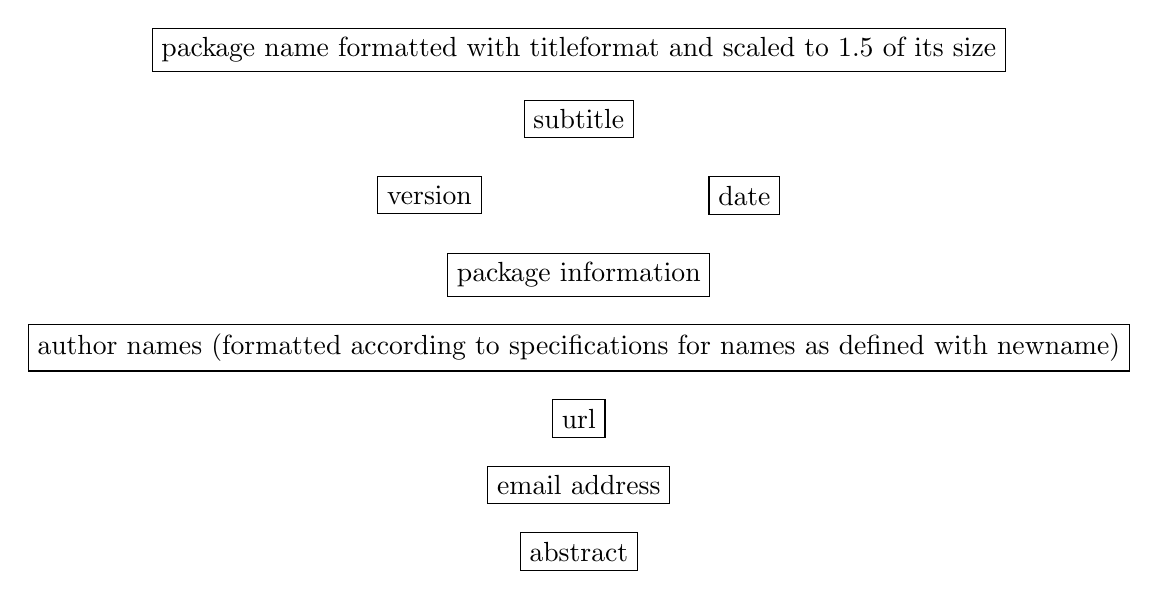
\begin{tikzpicture}[
      start chain=going below,
      node distance=1em,
      every node/.style={draw,align=center}
    ]
    \node[on chain] {package name formatted with \cs{titleformat} and scaled
      to 1.5 of its size} ;
    \node[on chain] {subtitle} ;
    \node[on chain,draw=none]
      {\tikz\draw (0,0) node[draw] {version} ++(4,0) node[draw] {date} ;} ;
    \node[on chain] {package information} ;
    \node[on chain] {author names (formatted according to specifications for
      names as defined with \cs{newname})} ;
    \node[on chain] {url} ;
    \node[on chain] {email address} ;
    \node[on chain] {abstract} ;
  \end{tikzpicture}
  \caption{Schematic sketch of the title page.}
  \label{fig:titlepage}
\end{figure}

\subsection{Predefined Preamble}\label{sec:preamble}
It is possible to load a part of my standard preamble automatically by
passing an option as class option.
\begin{options}
  \opt{load-preamble}
    Class option that preloads part of my custom preamble.
\end{options}

Using the option will include the following code:

\begin{sourcecode}
  \RequirePackage{ifxetex,ifluatex}
  \ifboolexpr{not bool{xetex} and not bool{luatex}}
    {\RequirePackage[T1]{fontenc}}
    {\RequirePackage{fontspec}}
  \RequirePackage[oldstyle]{libertine}
  % `libertinehologopatch' is not on CTAN, yet!
  % you can get it at https://bitbucket.org/cgnieder/libertinehologopatch
  \RequirePackage{libertinehologopatch}
  \RequirePackage[supstfm=libertinesups]{superiors}
  \RequirePackage{microtype}
  \ifboolexpr{not bool{xetex} and not bool{luatex}}
    {\RequirePackage[scaled=.83]{beramono}}
    {\setmonofont[Scale=MatchLowercase]{Bitstream Vera Sans Mono}}
  \RequirePackage{fnpct}
  \expandafter\RequirePackage\expandafter[\cnltx@babel@options]{babel}
  \renewcommand*\othersectionlevelsformat[3]{%
    \textcolor{cnltx}{#3\autodot}\enskip}
  \renewcommand*\partformat{%
    \textcolor{cnltx}{\partname~\thepart\autodot}}
  \deffootnote{2em}{1em}{\llap{\thefootnotemark. }}%
  \pagestyle{headings}
  \setcapindent{1.5em}
  \setkomafont{caption}{\cnltx@caption@font}
  \setkomafont{captionlabel}{\cnltx@captionlabel@font}
\end{sourcecode}

The effect of this preamble is demonstrated by the document you're reading at
this moment.

\subsection{Predefined Indexing}\label{sec:predefined-indexing}
\cnltxdoc\ allows the automated creation of an index.  This is done with the
help of the \pkg{imakeidx} package by \egreg.  To use this feature you have
two class options.  They cannot be set with \cs{setcnltx} but must be given as
class options.

\begin{options}
  \keybool{add-index}\Default{false}
    Enables the automatic creation of an index at the end of the document.
  \keybool{load-preamble+}\Default{false}
    This option has the same effect as adding both \option{load-preamble} and
    \option{add-index}.
\end{options}

Enabling the feature
\begin{itemize}
  \item loads the \needpackage{imakeidx} package,
  \item uses a given style file for the index that can be specified with the
    \option{index-style} option,
  \item sets a certain setup for the index that can be specified with the
    \option{index-setup} option and
  \item adds an index at the end of the document.
\end{itemize}

The following options are available to customize the appearance of the index:
\begin{options}
  \keyval{index-prologue}{text}
    Adds \meta{text} as index prologue between heading and the actual index.
  \keyval{index-space}{dimension}\Default{0pt}
    The vertical space between index prologue and index.
  \keyval{index-setup}{options}%
    \Default{othercode=\cs*{footnotesize},level=\cs*{section}}
    The options that are passed to \pkg{imakeidx}'s \cs*{indexsetup} command.
  \keyval{makeindex-setup}{options}\Default{columns=2,columnsep=1em}
    The options that are passed to the \cs*{makeindex} command.
  \keyval{index-style}{style file}\Default{cnltx.ist}
    The style file that is used for formatting the index.
\end{options}

The index style file \file{cnltx.ist} contains the following lines:
\inputsourcecode{cnltx.ist}

The feature is demonstrated by this document which does not contain a single
control sequence containing the string \code{index}!

\section{Predefined \pkg*{listings} and \pkg*{mdframed} Styles}

\subsection{\pkg*{mdframed}}

The source code environments (see section~\vref{sec:usage:examples}) all get a
frame with the help of the \pkg{mdframed} package.  For this a custom style is
defined called \code{cnltx}.  The options \option{frame-options} and
\option{add-frame-options} mentioned in section~\vref{sec:usage:examples}
manipulate this style.  It is predefined with these values:

\begin{sourcecode}
  \def\cnltx@mdframed@options
    {
      backgroundcolor = cnltxbg ,
      linecolor       = cnltx ,
      roundcorner     = 5pt
    }
\end{sourcecode}

\subsection{\pkg*{listings}}

The code of the source code environments (see
section~\vref{sec:usage:examples}) is formatted with the help of the
\pkg{listings} package.  A \pkg{listings} style is defined called
\code{cnltx}.  The options \option{add-cmds}, \option{add-silent-cmds},
\option{add-envs}, \option{add-silent-envs}, \option{listings-options} and
\option{add-listings-options} manipulate this style.  It is predefined as
follows:

\begin{sourcecode}
  \def\cnltx@listings@style{
    language         = [LaTeX]TeX,
    basicstyle       = {\sourceformat},
    numbers          = left,
    numberstyle      = \tiny,
    xleftmargin      = 1em,
    numbersep        = .5em,
    gobble           = \cnltx@gobble ,
    columns          = fullflexible,
    literate         =
      {ä}{{\"a}}1
      {ö}{{\"o}}1
      {ü}{{\"u}}1
      {Ä}{{\"A}}1
      {Ö}{{\"O}}1
      {Ü}{{\"U}}1
      {ß}{{\ss}}1 ,
    breaklines       = true,
    keepspaces       = true,
    breakindent      = 1em,
    commentstyle     = \color{comment},
    keywordstyle     = \color{cs},
    deletetexcs      =
      {
        a,o,u,A,O,U,
        begin,
        center,
        description,document,
        end,enumerate,
        figure,flushleft,flushright,
        itemize,
        otherlanguage,
        table,tabu,tabular
      },
    % \begin, \end:
    texcsstyle       = [2]\color{beginend},
    index            = [2][texcs2],
    indexstyle       = [2]\@gobble,
    moretexcs        = [2]{begin,end},
    % environments:
    texcsstyle       = [3]\color{env},
    index            = [3][texcs3],
    indexstyle       = [3]\@gobble,
    % control sequences:
    texcsstyle       = [4]\color{cs},
    index            = [4][texcs4],
    indexstyle       = [4]\@gobble ,
    % added control sequences:
    texcsstyle       = [5]\color{cs},
    index            = [5][texcs5],
    indexstyle       = [5]\indexcs,
    % added environments:
    texcsstyle       = [6]\color{env},
    index            = [6][texcs6],
    indexstyle       = [6]\envidx,
  }
\end{sourcecode}

\section{\PDF\ Strings and \pkg*{hyperref}}

Since the formatting and indexing commands \cs{cs}, \cs{env}, \cs{option},
\cs{pkg}, \cs{cls} and \cs{key} are robust they are ignored in \PDF\
strings.  For this reason you should \emph{only use the starred variants} in
places where \PDF\ bookmarks are built from such as section titles when you
use \pkg{hyperref}.  Since \cnltxdoc\ loads \pkg{hyperref} this means you
should do so, too, when you use \cnltxdoc.  This is important for two reasons:
\begin{enumerate}
  \item Indexing in strings that get written to the table of contents does
    noch make much sense, anyway, so the starred versions should be used in
    section titles even if you don't use \pkg{hyperref}.
  \item When \pkg{hyperref} is loaded the mentioned commands are disabled in
    \PDF\ strings in a way that \emph{expects} them to be followed by a star.
    This means leaving the star out will result in \code{doesn't match its
      definition} errors.
\end{enumerate}

\section{Predefined Colors and Color-Schemes}\label{sec:colors}
\subsection{Explicitly Defined Colors}\label{sec:colors:definitions}

The \cnltxbase\ package defines a number of colors:
\begin{colors}
  \colour{cnltxbrown}
    Per default used for the control sequences.
  \colour{cnltxblue}
    Unused per default.
  \colour{cnltxred}
    Per default used as base color in various places.
  \colour{cnltxgreen}
    Unused per default.
  \colour{cnltxgray}
    Per default used for formatting comments.
  \colour{cnltxyellow}
    Per default used for options.
  \colour{cnltxformalblue}
    Unused per default.
  \colour{cnltxformalred}
    Unused per default.
\end{colors}

\subsection{Actual Used Color Names and Color Schemes}

The colors defined in section~\vref{sec:colors:definitions} are not directly
used with those names.  Instead colors are used whose names describe their
function rather than the color.  For this the color names are mapped to actual
colors and saved as a coloring scheme.  There are currently three predefined
color schemes whose definitions are given below.  Those definitions also show
the actually used color names:

The `default' color scheme is defined as follows:
\begin{sourcecode}
  \cnltx@define@colorscheme{default}{
    cs          => cnltxbrown , % command sequences
    option      => cnltxyellow ,% options
    option      => cnltxyellow ,% modules
    comment     => cnltxgray ,  % comments
    beginend    => red ,        % \begin and \end
    env         => black ,      % environment names
    argument    => black ,      % argument delimiters
    meta        => black!80 ,   % arguments of \meta
    cnltx       => cnltxred ,   % base color
    cnltxbg     => white ,      % source code box background
    link        => black!90 ,   % hyperlinks
    versionnote => black!75     % versioning notes text 
  }
\end{sourcecode}

The `blue' color scheme is defined this way:
\begin{sourcecode}
  \cnltx@define@colorscheme{blue}{
    cs          => cnltxbrown ,
    option      => cnltxgreen ,
    module      => cnltxred ,
    comment     => cnltxgray ,
    beginend    => red ,
    env         => black ,
    argument    => black ,
    meta        => black!80 ,
    cnltx       => cnltxblue ,
    cnltxbg     => yellow!10 ,
    link        => cnltx ,
    versionnote => black!75
  }
\end{sourcecode}

Finally the `formal' color scheme is defined like this:
\begin{sourcecode}
  \cnltx@define@colorscheme{formal}{
    cs          => black ,
    option      => cnltxformalblue ,
    module      => cnltxblue ,
    comment     => cnltxgray ,
    beginend    => red ,
    env         => black ,
    argument    => black ,
    meta        => black!80 ,
    cnltx       => cnltxformalblue ,
    cnltxbg     => white ,
    link        => black!90 ,
    versionnote => black!75
  }
\end{sourcecode}

\section{Language Support}

\noindent\sinceversion{0.2}The \cnltxdoc\ and the \cnltxexample\ package both
rely on the \pkg{translations} package for providing some document language
dependent strings.  Currently only translations for English and German are
provided.  Others can be added and the existing ones changed with the
following command provided by the \pkg{translations} package:

\begin{commands}
  \command{DeclareTranslation}[\marg{language}\marg{keyword}\marg{translation}]
    Provide translations for the string identified by the \textsc{id}
    \meta{keyword}.
\end{commands}

The defined strings are listed in table~\vref{tab:language:strings}.  They are
used in indexing strings and in different parts of the document.

\begin{table}[htb]
  \centering\renewcommand\arraystretch{1.3}
  \caption{Overview over available internationalization key words.}
  \label{tab:language:strings}
  \begin{tabular}{
      l
      >{\ttfamily}l
      >{\RaggedRight}p{.25\linewidth}
      >{\RaggedRight}p{.25\linewidth}
    }
    \toprule
      Package       & key word          & English version & German version\\
    \midrule
      \cnltxexample & cnltx-package &
        \GetTranslation{cnltx-package} &
        \GetTranslationFor{German}{cnltx-package} \\
      \cnltxexample & cnltx-class &
        \GetTranslation{cnltx-class} &
        \GetTranslationFor{German}{cnltx-class} \\
      \cnltxexample & cnltx-environment &
        \GetTranslation{cnltx-environment} &
        \GetTranslationFor{German}{cnltx-environment} \\
      \cnltxdoc     & cnltx-default &
        \GetTranslation{cnltx-default} &
        \GetTranslationFor{German}{cnltx-default} \\
      \cnltxdoc     & cnltx-empty &
        \GetTranslation{cnltx-empty} &
        \GetTranslationFor{German}{cnltx-empty} \\
      \cnltxdoc     & cnltx-required &
        \GetTranslation{cnltx-required} &
        \GetTranslationFor{German}{cnltx-required} \\
      \cnltxdoc     & cnltx-toc &
        \GetTranslation{cnltx-toc} &
        \GetTranslationFor{German}{cnltx-toc} \\
      \cnltxdoc     & cnltx-license &
        \GetTranslation{cnltx-license} &
        \GetTranslationFor{German}{cnltx-license}\\
      \cnltxdoc     & cnltx-introduced &
        \GetTranslation{cnltx-introduced} &
        \GetTranslationFor{German}{cnltx-introduced} \\
      \cnltxdoc     & cnltx-changed &
        \GetTranslation{cnltx-changed} &
        \GetTranslationFor{German}{cnltx-changed} \\
      \cnltxdoc     & cnltx-f. &
        \GetTranslation{cnltx-f.} &
        \GetTranslationFor{German}{cnltx-f.} \\
      \cnltxdoc     & cnltx-ff. &
        \GetTranslation{cnltx-ff.} &
        \GetTranslationFor{German}{cnltx-ff.} \\
    \bottomrule
  \end{tabular}
\end{table}

\part{Appendix}
\appendix

\section{Internal Helper Commands}

The commands in this section are only described for the sake of completeness.
They are not meant to be used in a document.

\subsection{Defined by \cnltxbase}

Especially \cnltxbase\ defines some useful helper macros that are also used by
the other packages and classes.

\begin{commands}
  \command{cnltx\at\at date}
    The creation date of the current version of the bundle.
  \command{cnltx\at\at version}
    The version number of the bundle.
  \command{cnltx\at\at info}
    The short description of the bundle.
  \command{cnltx\at create\at message}%
    [\sarg\marg{module}\Marg{\choices{Error,Warning,WarningNoLine,Info}}]
    \changedversion{0.2}Create suiting error and warning messaging commands
    for the module \meta{module}.  The starred version creates messages for a
    class the un-starred version messages for a package.
  \command{cnltx\at base\at error}[\marg{message}]
    Issue an error message using \cs*{PackageError}\Marg{cnltx-base}.
  \command{cnltx\at base\at warning}[\marg{message}]
    Issue a warning message using \cs*{PackageWarning}\Marg{cnltx-base}.
    \command{cnltx\at base\at warningnoline}[\marg{message}]
    Issue a warning message using \cs*{PackageWarningNoLine}\Marg{cnltx-base}.
  \command{cnltx\at base\at info}[\marg{message}]
    Issue a message using \cs*{PackageInfo}\Marg{cnltx-base}.
  \command{cnltx\at par}
    Expands to \cs*{par}.  Sometimes you need to smuggle a \cs*{par} in a
    short macro \ldots
  \command{cnltx\at ifsym}[\marg{token}\marg{true}\marg{false}]
    A generic version of \LaTeX's \cs*{@ifstar} that checks if \meta{token}
    follows if the input stream.  If yes it is removed and \meta{true} is
    placed in the input stream else \meta{false}.
  \command{cnltx\at ifdash}[\marg{true}\marg{false}]
    A wrapper for \verbcode+\cnltx@ifsym{-}+.
  \command{cnltx\at ifbang}[\marg{true}\marg{false}]
    \sinceversion{0.3}A wrapper for \verbcode+\cnltx@ifsym{!}+.
  \command{cnltx\at expand\at arg}[\marg{cs}\marg{macro}]
    Expands \meta{macro} once before it is passed as argument to \meta{cs}.
  \command{cnltx\at fullexpand\at arg}[\marg{cs}\marg{argument}]
    Exhaustive expansion of \meta{argument} before it is passed as argument to
    \meta{cs}.
  \command{cnltx\at fullexpand\at twoargs}[\marg{cs}\marg{argument1}\marg{argument2}]
    Exhaustive expansion of \meta{argument1} and \meta{argument2} before
    they're passed as argumenst to \meta{cs}.  This is an alias of the kernel
    command \cs*{@expandtwoargs} defined for the sake of consistency.
  \command{cnltx\at stripbs}
    A shortcut for \verbcode+\expandafter\@gobble\string+.
  \command{cnltx\at if\at in}[\marg{tokenlist}\marg{search}\marg{true}\marg{false}]
    Places \meta{true} in the input stream if \meta{search} is found in
    \meta{tokenlist} and \meta{false} if it isn't.
  \command{cnltx\at replace\at once}[\marg{cs}\marg{search}\marg{replace}]
    Replaces the first occurence of \meta{search} in the first expansion of
    \meta{cs} with \meta{replace}.
  \command{cnltx\at long\at replace\at once}[\marg{cs}\marg{search}\marg{replace}]
    \sinceversion{0.3}The same as \cs{cnltx\at replace\at once} but \meta{cs}
    will be redefined with \cs*{long}.
  \command{cnltx\at replace\at all}[\marg{cs}\marg{search}\marg{replace}]
    Replaces all occurences of \meta{search} in the first expansion of
    \meta{cs} with \meta{replace}.
  \command{cnltx\at long\at replace\at all}[\marg{cs}\marg{search}\marg{replace}]
    \sinceversion{0.3}The same as \cs{cnltx\at replace\at all} but \meta{cs}
    will be redefined with \cs*{long}.
  \command{cnltx\at remove\at once}[\marg{cs}\marg{search}]
    \sinceversion{0.3}Removes the first occurence of \meta{search} in the
    first expansion of \meta{cs}.
  \command{cnltx\at long\at remove\at once}[\marg{cs}\marg{search}]
    \sinceversion{0.3}The same as \cs{cnltx\at remove\at once} but \meta{cs}
    will be redefined with \cs*{long}.
  \command{cnltx\at remove\at all}[\marg{cs}\marg{search}]
    \sinceversion{0.3}Removes all occurences of \meta{search} in the first
    expansion of \meta{cs}.
  \command{cnltx\at long\at remove\at all}[\marg{cs}\marg{search}]
    \sinceversion{0.3}The same as \cs{cnltx\at remove\at all} but \meta{cs}
    will be redefined with \cs*{long}.
  \command{cnltx\at define\at colorscheme}[\marg{name}\marg{scheme definition}]
    Command that can be used to define a color scheme.
\end{commands}

\subsection{Defined by \cnltxexample}

\begin{commands}
  \command{cnltx\at example\at error}[\marg{message}]
    Issue an error message using \cs*{PackageError}\Marg{cnltx-example}.
  \command{cnltx\at example\at warning}[\marg{message}]
    Issue a warning message using \cs*{PackageWarning}\Marg{cnltx-example}.
    \command{cnltx\at example\at warningnoline}[\marg{message}]
    Issue a warning message using \cs*{PackageWarningNoLine}\Marg{cnltx-example}.
  \command{cnltx\at example\at info}[\marg{message}]
    Issue a message using \cs*{PackageInfo}\Marg{cnltx-example}.
  \command{cnltxat}
    Robust command that typesets `\at' with category code 11.  An @ in command
    names confuses the indexing of the command names.  Either one uses another
    symbol for makeindex's ``actual'' recognition and also tells \pkg{idxcmds}
    about it or one uses \cs{cnltxat} in \cs{cs} and friends.  For the
    sake of convenience you can define a command like \cs*{at} that expands to
    it\footnote{This is important.  If you \cs*{let} it to \cs{cnltxat} index
      entries may be sorted differently! Remember: \cs{cnltxat} is robust.}.
    In order not to overwrite any such existing macro it is not defined by
    \cnltxexample.  This document for example defines
    \verbcode+\def\at{\cnltxat}+.
  \command{cnltxletterat}
    An alias of \cs{cnltxat}.
  \command{cnltxotherat}
    The same as \cs{cnltxat} but with a `\at' with category code 12.
  \command{cnltxbang}
    The same as \cs{cnltxotherat} except that it contains a `\bang'.
  \command{cnltxequal}
    The same as \cs{cnltxotherat} except that it contains a `\equal'.
  \command{cnltx\at isvalue}
    Used in definitions of the key/value option typesetting commands.  Inserts
    a \code{=} with some stretchable space around and a legal break-point
    after it.
  \command{indexcs}
    Version of \cs{csidx} that takes care of a \cs*{textcompwordmark} inserted
    by listings. Also replaces all occurences of @ with category code 11 or 12
    with \cs{cnltxat}. Used to index commands in the \env{sourcecode} and
    \env{example} environments that have been added with \option{add-cmds}.
  \command{newarg}[\oarg{arg formatting}\marg{cs}\marg{left delim}\marg{right delim}]%
    \Default{\cs{meta}}
    \changedversion{0.2}Command used to define the argument commands:
    \verbcode+\newarg\marg{\{}{\}}+.  The optional argument determines how the
    argument of the new command will be formatted.  This is done with
    \cs{meta} per default.  \verbcode+\newarg[\code]\Marg{\{}{\}}+
  \command{MakePercentComment}
    Sets the category code of \code{\%} to 14.
  \command{cnltx\at copyablespace}
    Prints a space that is also copyable.  Uses the \pkg{accsupp} package by
    \oberdiek.
  \command{cnltx\at mdframed\at options}
    Predefined option list for the \pkg{mdframed} style \code{cnltx}.
  \command{cnltx\at listings\at style}
    Predefined option list for the \pkg{listings} style \code{cnltx}.
\end{commands}

\subsection{Defined by \cnltxtools}

\begin{commands}
  \command{cnltx\at tools\at error}[\marg{message}]
    Issue an error message using \cs*{PackageError}\Marg{cnltx-tools}.
  \command{cnltx\at tools\at warning}[\marg{message}]
    Issue a warning message using \cs*{PackageWarning}\Marg{cnltx-tools}.
    \command{cnltx\at tools\at warningnoline}[\marg{message}]
    Issue a warning message using \cs*{PackageWarningNoLine}\Marg{cnltx-tools}.
  \command{cnltx\at tools\at info}[\marg{message}]
    Issue a message using \cs*{PackageInfo}\Marg{cnltx-tools}.
  \command{cnltx\at accsupp}[\marg{actual text}\marg{additional
    options}\marg{\TeX\ text}]
    A wrapper for package \pkg{accsupp}'s \cs*{BeginAccSupp}\Marg{ActualText
      = \meta{actual text}} \meta{\TeX\ text} \cs*{EndAccSupp}\marg{}.
\end{commands}
  
\subsection{Defined by \cnltxdoc}

\begin{commands}
  \command{cnltx\at doc\at error}[\marg{message}]
    Issue an error message using \cs*{ClassError}\Marg{cnltx-doc}.
  \command{cnltx\at doc\at warning}[\marg{message}]
    Issue a warning message using \cs*{ClassWarning}\Marg{cnltx-doc}.
    \command{cnltx\at doc\at warningnoline}[\marg{message}]
    Issue a warning message using \cs*{ClassWarningNoLine}\Marg{cnltx-doc}.
  \command{cnltx\at doc\at info}[\marg{message}]
    Issue a message using \cs*{ClassInfo}\Marg{cnltx-doc}.
  \command{cnltx\at getfileinfo}[\marg{file name}\marg{file extension}]
    Extract the date, version and background information for a package or a
    class.
  \command{cnltx\at version\at note}[\marg{note}]
    Command that is used for the versioning notes interally.  Sets
    \cs*{reversemarginpar} and then writes the note \meta{note} to the margin
    with corresponding formatting.
\end{commands}
\begin{environments}
  \environment{cnltxlist}
    The list environment that is used by the environments \env{commands},
    \env{options} and \env{environments}.
\end{environments}

\subsection{Defined by \cnltxcsnames}

\begin{commands}
  \command{cnltx\at predefined\at control\at sequences}
    A comma-separated list of predefined `silent' control sequence names.
  \command{cnltx\at predefined\at environments}
    A comma-separated list of predefined `silent' environment names.
  \command{listsilentcmds}
    Prints all known control sequence names formatted and separated with a
    comma.
  \command{listsilentenvs}
    Prints all known environment names formatted and separated with a
    comma.
\end{commands}

\section{List of Known \LaTeX\ Control Sequences}\label{sec:known:csnames}

Below are listed all \emph{predefined} control sequence names that are treated
as ``silent'' names by \cnltx, that is, those defined by \cnltxcsnames.  You
may notice that the list does not cover all control sequences that are
formatted.  That is because \pkg{listings} already has a number of known
control sequence names.  This list probably overlaps with those on some parts,
though.

\begin{multicols}{3}
  \RaggedRight\listsilentcmds
\end{multicols}

\section{List of Known \LaTeX\  Environments}\label{sec:known:environments}

Below are listed all \emph{predefined} control sequence names that are treated
as ``silent'' names by \cnltx, that is, those defined by \cnltxcsnames.

\begin{multicols}{3}
  \RaggedRight\listsilentenvs
\end{multicols}

\end{document}
